\documentclass[aspectratio=169]{beamer}

\usepackage[utf8]{inputenc}
%\usepackage[spanish]{babel}
\usepackage{graphicx}
\usepackage{booktabs}
\usepackage{ragged2e}
\usepackage{minted}
\usepackage{xcolor}
\usepackage{algorithm}
\usepackage{algorithmic}
\usepackage{listings}
\usepackage{tikz}
\usepackage[style=authoryear, backend=biber]{biblatex}
\addbibresource{Class02.bib}
\usetikzlibrary{arrows.meta,positioning,fit,shapes.symbols}
\usetikzlibrary{arrows,shapes}
\definecolor{LightGray}{gray}{0.975}
\definecolor{links}{HTML}{2A1B81}
\hypersetup{colorlinks,linkcolor=,urlcolor=blue}
\AtBeginEnvironment{minted}{%
  \renewcommand{\fcolorbox}[4][]{#4}}

\usefonttheme{serif}

\usepackage{listings}
\lstdefinestyle{myCustomSQLStyle}{
  language=SQL,
  numbers=left,
  stepnumber=1,
  numbersep=10pt,
  tabsize=4,
  frame=single,
  backgroundcolor=\color{LightGray},
  breaklines=true,
  showspaces=false,
  showstringspaces=false
}

\newcommand\Wider[2][18mm]{%
    \makebox[\linewidth][c]{%
        \begin{minipage}{\dimexpr\textwidth+#1\relax}
            \raggedright#2
        \end{minipage}%
    }%
}
\newcommand\userinput[1]{\textbf{#1}}

\title[Class 06]{Change Detection \& Image Time Series Analysis}
\author{Lillesand, Chipman \& Kiefer, 2015.}
\date{\today}

% Remove navigation symbols...
\setbeamertemplate{navigation symbols}{}

\defbeamertemplate*{footline}{shadow theme}{
    \leavevmode
    \hbox{
        \begin{beamercolorbox}[
                wd =        0.33\paperwidth,
                ht =        2.5ex,
                dp =        1.125ex,
                leftskip =  0.3cm plus1fil,
                rightskip = 0.3cm
            ]{author in head/foot}
            \flushleft EDT
        \end{beamercolorbox}
        \begin{beamercolorbox}[
                wd =        0.33\paperwidth,
                ht =        2.5ex,
                dp =        1.125ex,
                leftskip =  0.3cm plus1fil,
                rightskip = 0.3cm
            ]{author in head/foot}
            \insertshorttitle
        \end{beamercolorbox}
        \begin{beamercolorbox}[
                wd =        0.33\paperwidth,
                ht =        2.5ex,
                dp =        1.125ex,
                leftskip =  0.3cm plus1fil,
                rightskip = 0.3cm
            ]{title in head/foot}
            \hfill \insertframenumber\,/\,\inserttotalframenumber%
        \end{beamercolorbox}
    }
}

\AtBeginSection[]
{
     \begin{frame}<beamer>
     \frametitle{Plan}
     \tableofcontents[currentsection]
     \end{frame}
}

\begin{document}

\frame{\titlepage}

\begin{frame}{Outline}
    \tableofcontents
\end{frame}

\section{Change Detection}

\subsection{Introduction}

\begin{frame}{What is Change Detection?}
    \begin{itemize}
        \item \textbf{Definition:} The process of identifying and characterizing differences in conditions at different points in time.
        \item \textbf{Value:} One of the most powerful advantages of remote sensing is preserving a temporal record.
        \item \textbf{Scales of Change:}
        \begin{itemize}
            \item \textit{Short-term:} Vehicle or animal movement.
            \item \textit{Long-term:} Urban development or desertification.
        \end{itemize}
    \end{itemize}
\end{frame}

\subsection{Requirements}

\begin{frame}{Technical Requirements}
    To minimize ``false'' changes, data should ideally be acquired using:
    \begin{itemize}
        \item Same or similar \textbf{sensors}.
        \item Identical \textbf{spatial resolution} and viewing geometry.
        \item Matching \textbf{spectral bands} and radiometric resolution.
        \item Consistent \textbf{time of day} to maintain sun angle.
        \item \textbf{Anniversary dates:} Preferred for long-term (>1 year) studies to minimize seasonal differences.
    \end{itemize}
\end{frame}

\begin{frame}{Registration and Environmental Factors}
    \begin{block}{Spatial Accuracy}
        Effective detection requires accurate registration, ideally within $\frac{1}{4}$ to $\frac{1}{2}$ pixel. Misregistration $>1$ pixel causes significant errors.
    \end{block}
    \begin{itemize}
        \item \textbf{Environmental Influences:}
        \begin{itemize}
            \item Atmospheric effects.
            \item Water levels and tidal stages.
            \item Soil moisture and wind.
            \item Plant phenology (season-to-season biological changes).
        \end{itemize}
    \end{itemize}
\end{frame}

\subsection{Post-classification}

\begin{frame}{Method 1: Post-classification Comparison}
    \begin{itemize}
        \item \textbf{Process:} Two dates are independently classified and registered.
        \item \textbf{Mechanism:} Pixels that changed class (e.g., Class A $\rightarrow$ Class B) are identified.
        \item \textbf{Pros:} Provides specific ``from-to'' change maps and statistics.
        \item \textbf{Cons:} Accuracy depends on the precision of both independent classifications; \textbf{errors are compounded}.
    \end{itemize}
\end{frame}

\begin{frame}{Post-classification change detection}
    \centering
    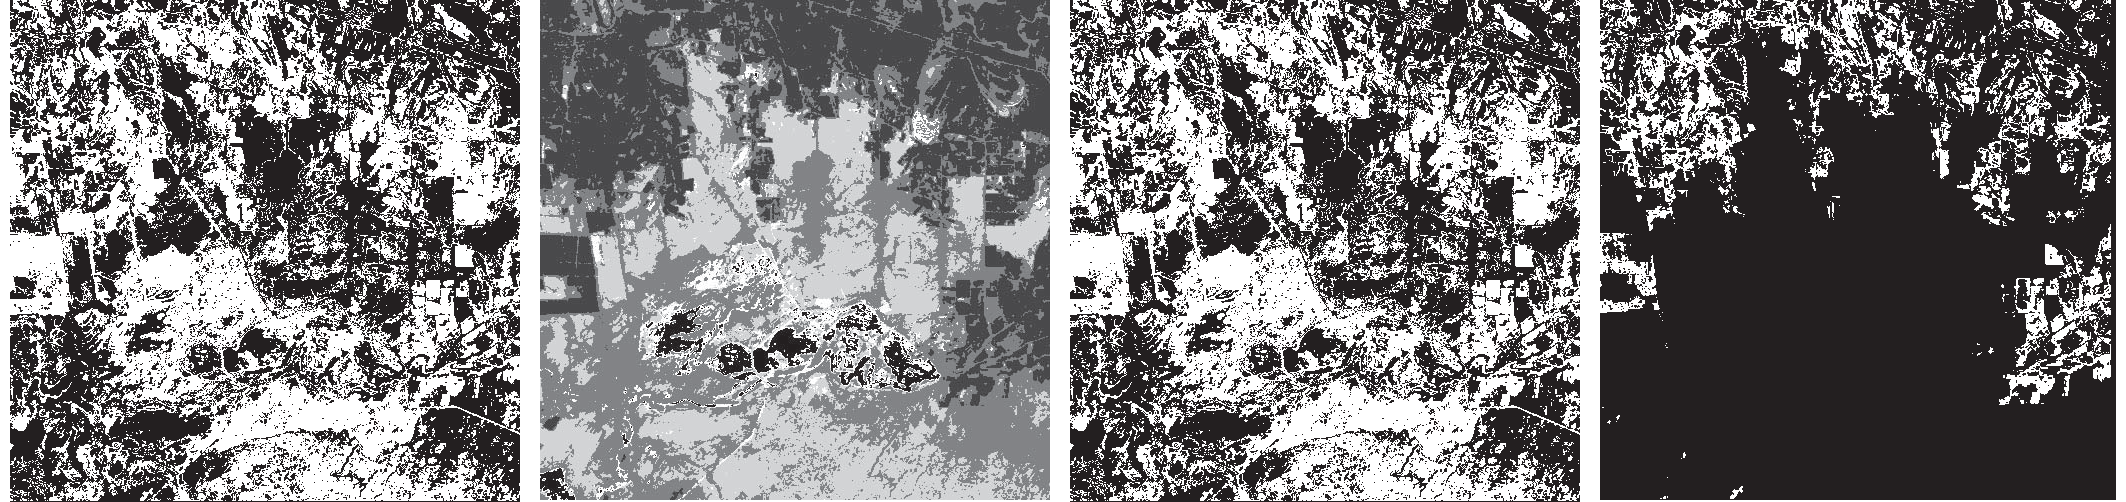
\includegraphics[width=\textwidth]{figures/fig55.png}
    (a) classification on date 1; (b) classification on date 2; (c) all change pixels highlighted in white; (d) only pixels that changed from class ``shrubland'' to class ``agriculture''.
\end{frame}

\begin{frame}{Method 2: Classification of Multitemporal Data}
    \begin{itemize}
        \item \textbf{The ``Stacking'' Approach:} Spectral bands from Date 1 and Date 2 are combined into a single data set (e.g., two 4-band images become one 8-band image).
        \item \textbf{Analysis:} Supervised or unsupervised classification is run on the stack.
        \item \textbf{Classes:} Resulting classes represent either stable land cover or specific ``change classes''.
        \item \textbf{Challenge:} High dimensionality and potential redundancy in information.
    \end{itemize}
\end{frame}

\begin{frame}{Method 3: Principal Components Analysis}
    \begin{itemize}
        \item \textbf{Approach:} Multiple dates are registered into a multiband image, and PCA is computed.
        \item \textbf{Change Detection:} Uncorrelated principal components often highlight areas of change (e.g., detecting tornado damage paths).
        \item \textbf{Advantages:} Excellent for identifying distinct physical changes.
        \item \textbf{Disadvantages:} It is often difficult to interpret the specific nature of the change.
    \end{itemize}
\end{frame}

\begin{frame}{Method 4: Temporal Image Differencing}
    \begin{itemize}
        \item \textbf{Calculation:} Digital Numbers (DNs) from Date 1 are subtracted from Date 2.
        \item \textbf{Range:} For 8-bit images, results range from $-255$ to $+255$.
        \item \textbf{Interpretation:}
        \begin{itemize}
            \item \textit{Near Zero:} No change (mid-gray tone).
            \item \textit{Positive/Negative:} Large changes (bright or dark tones).
        \end{itemize}
        \item \textbf{Display:} A constant (e.g., 127 or 255) is often added for visualization.
    \end{itemize}
\end{frame}

\begin{frame}{Method 5: Temporal Image Ratioing}
    \begin{itemize}
        \item \textbf{Calculation:} Computing the ratio of data between two dates.
        \item \textbf{Logic:} Areas of no change result in a ratio of $1$.
        \item \textbf{Advantage:} Tends to normalize data for extraneous factors like \textbf{sun angle} and \textbf{shadows}.
        \item Like differencing, results are typically scaled for display.
    \end{itemize}
\end{frame}

\begin{frame}{Temporal image differencing}
    \centering
    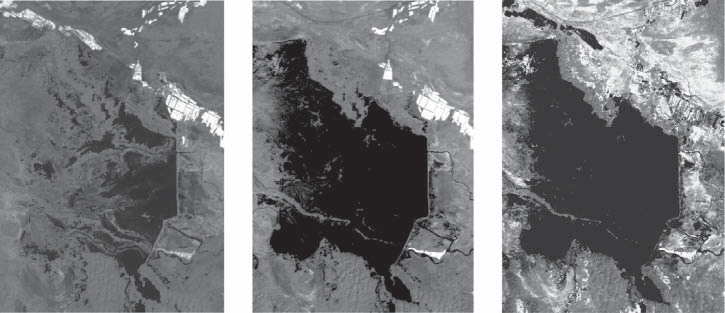
\includegraphics[width=\textwidth]{figures/fig56.png}
    (a) near-IR band from date 1; (b) near-IR band from date 2; (c) difference of (b) minus (a).
\end{frame}

\subsection{Change Thresholds}

\begin{frame}{Determining ``Change'' Thresholds}
    \begin{itemize}
        \item \textbf{The Threshold:} Analysts must find a ``change-no change'' threshold by looking at the \textbf{histogram tails} of differenced or ratioed data.
        \item \textbf{Enhancements:} Rather than raw DNs, analysts often use:
        \begin{itemize}
            \item Atmospheric/Illumination corrections.
            \item Radiance or Reflectance values.
            \item Vegetation components or Linear Regression models.
        \end{itemize}
    \end{itemize}
\end{frame}

\begin{frame}{Method 6: Change Vector Analysis}
    \begin{itemize}
        \item \textbf{Concept:} A conceptual extension of differencing using two or more spectral variables.
        \item \textbf{The Vector:} Describes both \textbf{magnitude} and \textbf{direction} of spectral change.
        \item \textbf{Applications:}
        \begin{itemize}
            \item Magnitude threshold determines if a change occurred.
            \item Direction identifies the \textit{type} of change (e.g., clearing vs. regrowth).
        \end{itemize}
    \end{itemize}
\end{frame}

\begin{frame}{Spectral change vector analysis}
    \centering
    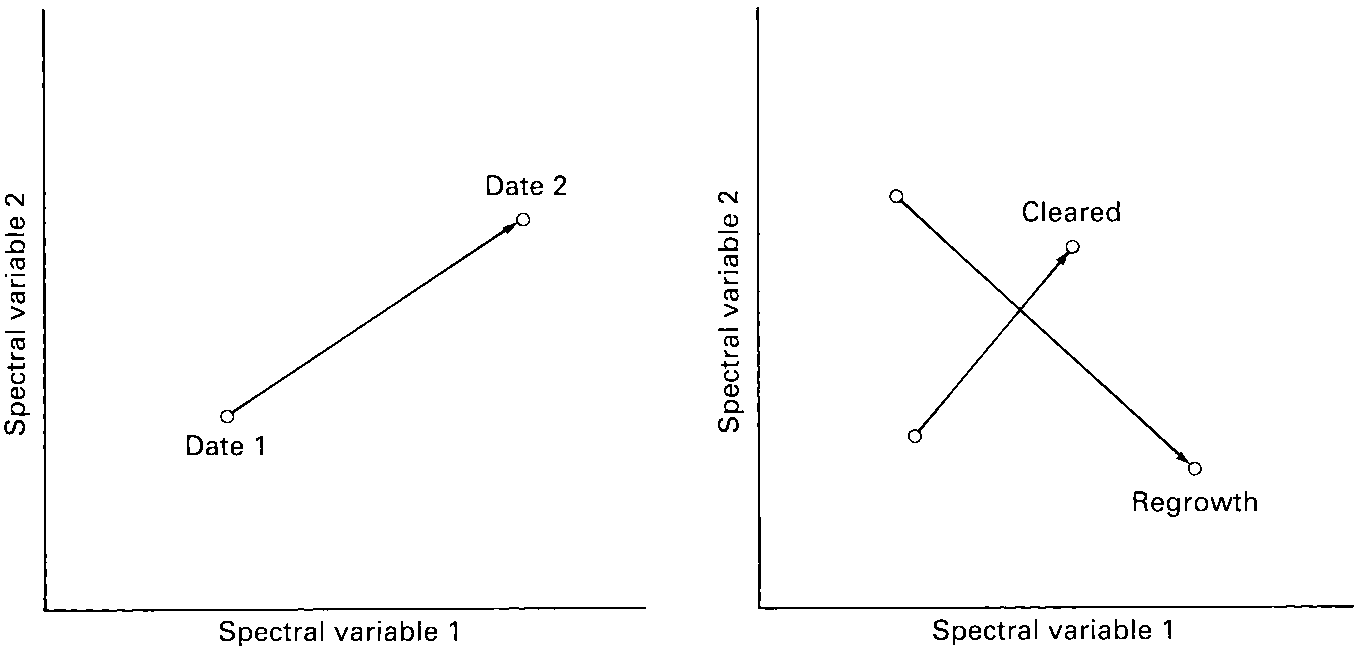
\includegraphics[width=0.9\textwidth]{figures/fig57.png} \\
    (a) spectral change vector observed for a single land cover type; (b) length and direction of spectral change vectors for hypothetical ``cleared'' and ``regrowth'' areas.
\end{frame}

\subsection{Binary Masking}

\begin{frame}{Efficiency and Automation}
    \begin{itemize}
        \item \textbf{Binary Masking:} Create a change-vs-no-change mask (via differencing/ratioing) to focus classification only on areas where change occurred.
        \item \textbf{Conclusion:} Change detection is increasingly vital due to the massive volume of data from:
        \begin{itemize}
            \item Expanded satellite constellations.
            \item Airborne platforms.
            \item Rapidly expanding UAV (drone) technology.
        \end{itemize}
        \item \textbf{Future:} Emphasis on \textbf{automated} methods to interpret the significance of changes.
    \end{itemize}
\end{frame}

\section{Image Time Series Analysis}

\subsection{Introduction}

\begin{frame}{The Rise of Time Series Analysis}
    \begin{itemize}
        \item \textbf{Beyond Snapshots:} Traditional change detection uses pairs of images; Time Series Analysis uses hundreds.
        \item \textbf{Global Monitoring Systems:} Enabled by sensors like \textbf{AVHRR} and \textbf{MODIS}.
        \item \textbf{Data Richness:} Daily to monthly intervals over decades.
        \item \textbf{Purpose:} Captures seasonal to decadal variations in:
        \begin{itemize}
            \item Agricultural cycles.
            \item Ecological health.
            \item Hydrological systems.
        \end{itemize}
    \end{itemize}
\end{frame}

\begin{frame}{What is a Temporal Signature?}
    \begin{itemize}
        \item Every pixel is a ``link in a long chain'' of imagery (e.g., 544 consecutive MODIS images).
        \item \textbf{Extraction:} By tracking a single pixel over time, we create a \textbf{temporal signature}.
    \end{itemize}
    \vspace{0.5cm}
    \begin{block}{Case Study: Xinjiang Region}
        \begin{itemize}
            \item \textbf{Agriculture:} Sharp cyclical peaks (planting to harvest).
            \item \textbf{Desert:} A flat, near-zero line.
            \item \textbf{Flooded Shrubland:} Sudden spikes in greenness followed by gradual decay.
        \end{itemize}
    \end{block}
\end{frame}

\begin{frame}{Time Series Example I}
    \centering
    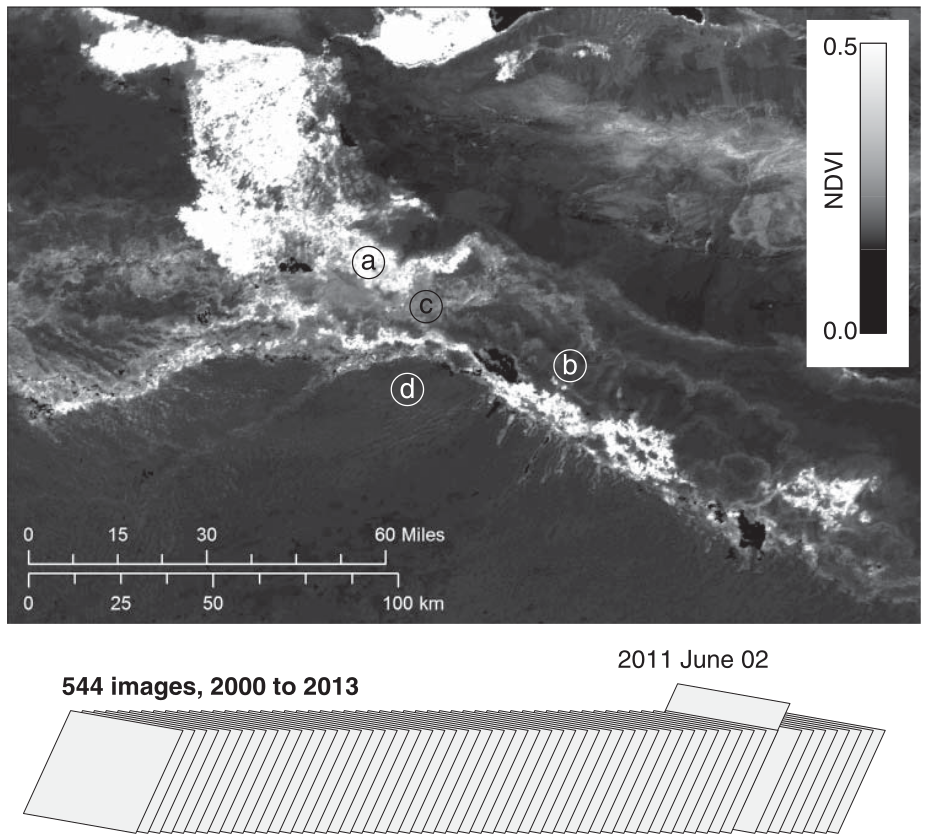
\includegraphics[width=0.575\textwidth]{figures/fig58.png} \\
    \tiny MODIS NDVI imagery extracted from a time series of 544 images for the Tarim River area in Xinjiang, China, from February 2000 through February 2013. Labeled points (a–d) are sources for time-series graphs shown in next figure.
\end{frame}

\begin{frame}{Time Series Example II}
    \centering
    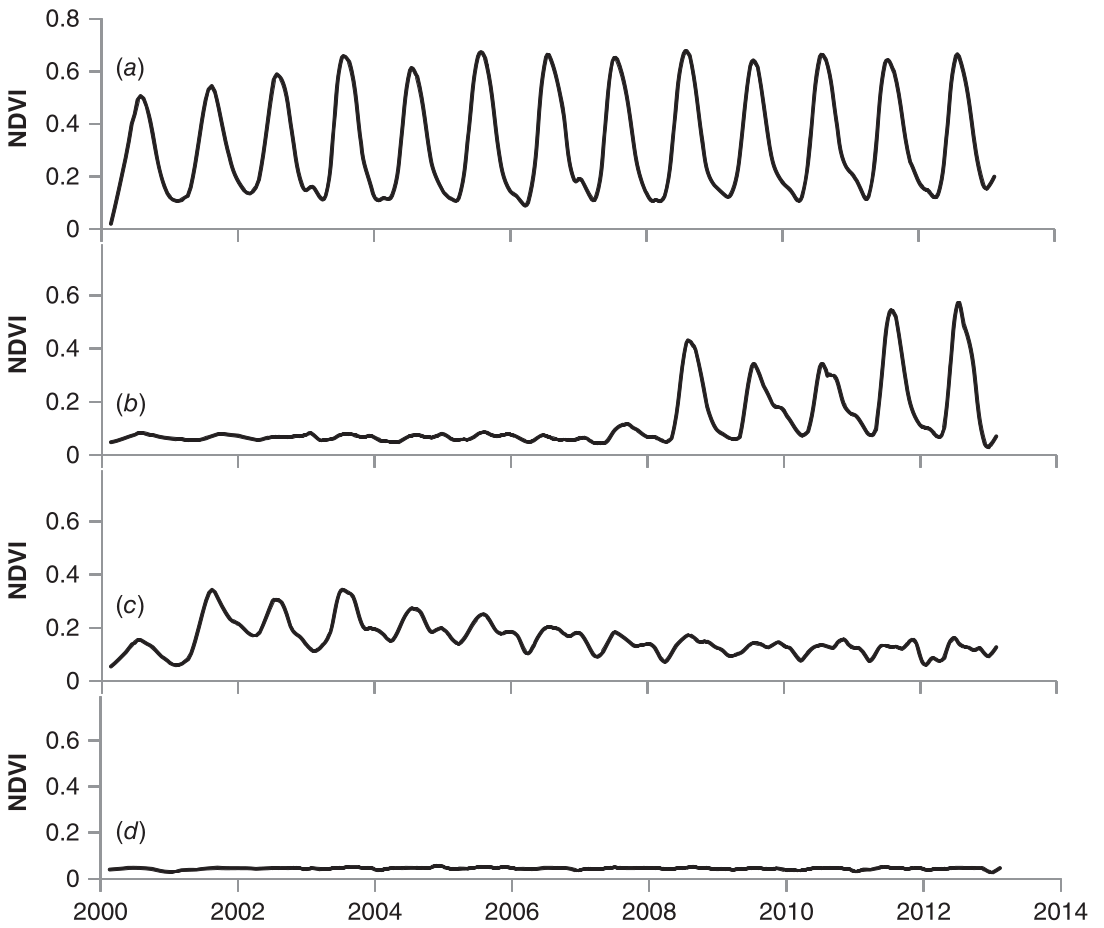
\includegraphics[width=0.6\textwidth]{figures/fig59} \\
    \tiny Time-series plots of previous MODIS NDVI figure: (a) established cotton farms; (b) new cotton farms; (c) tamarisk shrubland following an episode of flooding; (d) sand dunes.
\end{frame}

\subsection{Landscape Phenology}

\begin{frame}{Landscape Phenology}
    \begin{itemize}
        \item \textbf{Definition:} The study of spatial-temporal variations in vegetation indices (like NDVI or EVI) across the landscape.
        \item \textbf{Key Research Areas:}
        \begin{itemize}
            \item Linkages between climate and ecosystems.
            \item Agricultural yield forecasting.
            \item Hydrologic monitoring and snow/ice cover changes.
        \end{itemize}
    \end{itemize}
    \begin{quote}
        \textit{``It is the pulse of the annual cycle of green-up and senescence''}.
    \end{quote}
\end{frame}

\begin{frame}{Case Study: Northern Tanzania (2000--2011)}
    Using \textit{the Enhanced Vegetation Index (EVI)} to understand savannas:
    \begin{itemize}
        \item \textbf{Long-term Mean:} Shows average vegetation density.
        \item \textbf{Linear Decadal Trends:} Identifies areas with permanent gains (greening) or losses (browning) in vegetation.
        \item \textbf{Seasonal Amplitude:} Measures the ``peak-to-trough'' variation (high in seasonal grasslands, low in stable forests).
        \item \textbf{Application:} Understanding movements of migratory ungulates like wildebeest.
    \end{itemize}
\end{frame}

\begin{frame}{Northern Tanzania (2000--2011)}
    \centering
    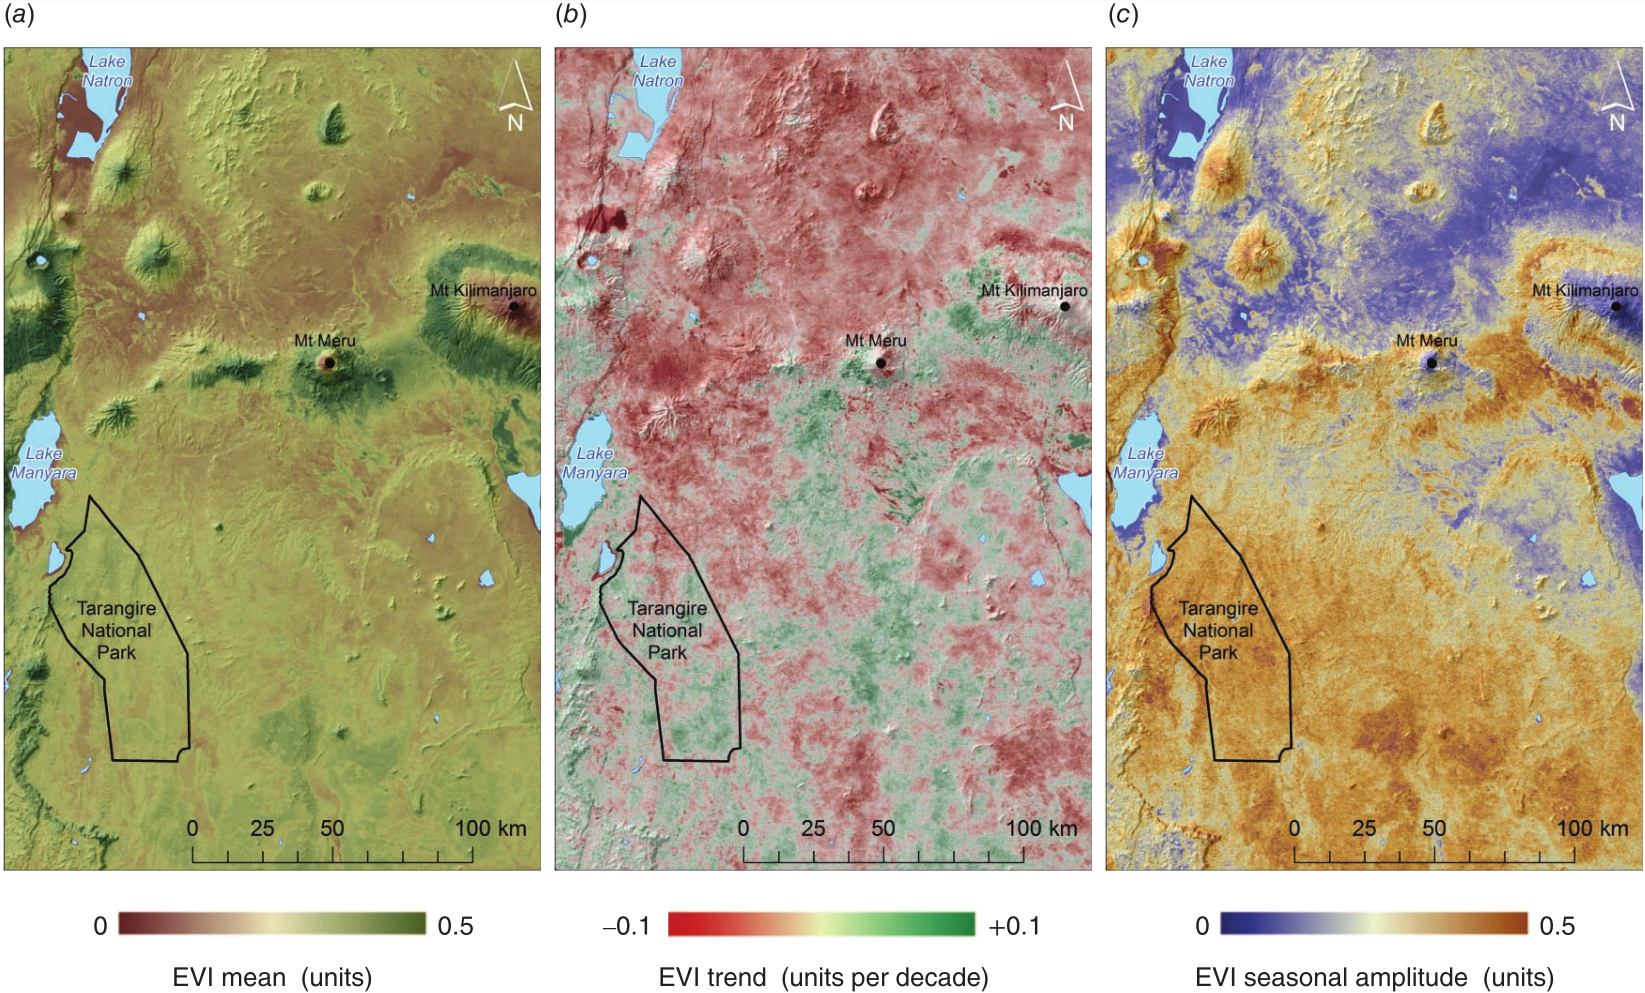
\includegraphics[width=0.875\textwidth]{figures/plate32} \\
    \tiny Time series of MODIS EVI data. (a) Long-term mean. (b) Decadal trend. (c) Amplitude of seasonal cycle.
\end{frame}

\subsection{A Greenness Profile}

\begin{frame}{Modeling Spectral Response Patterns}
    Scientists use physical modeling to classify crops and estimate productivity.
    \begin{itemize}
        \item \textbf{Annual Crops:} Follow a \textbf{sigmoidal} time behavior.
        \item \textbf{Soil Background ($G_0$):} Generally remains constant.
    \end{itemize}
    \vspace{0.3cm}

    \vspace{0.3cm}
    \begin{block}{The Sigmoidal Equation}
        Greenness at time $t$ is modeled using peak values and inflection points.
    \end{block}
\end{frame}

\begin{frame}{Dimensionality Reduction in Time Series}
    Instead of using 50+ raw images, we can characterize a season using three primary features:
    \begin{enumerate}
        \item $G_m$: \textbf{Peak Greenness} (The maximum intensity).
        \item $t_p$: \textbf{Time of Peak Greenness} (When it occurs).
        \item $\sigma$: \textbf{Width of the Profile} (Duration between inflection points $t_1$ and $t_2$).
    \end{enumerate}
    \begin{itemize}
        \item These three variables account for \textbf{$>95\%$} of the information in the original temporal data.
    \end{itemize}
\end{frame}

\begin{frame}{Temporal profile model for greenness}
    \centering
    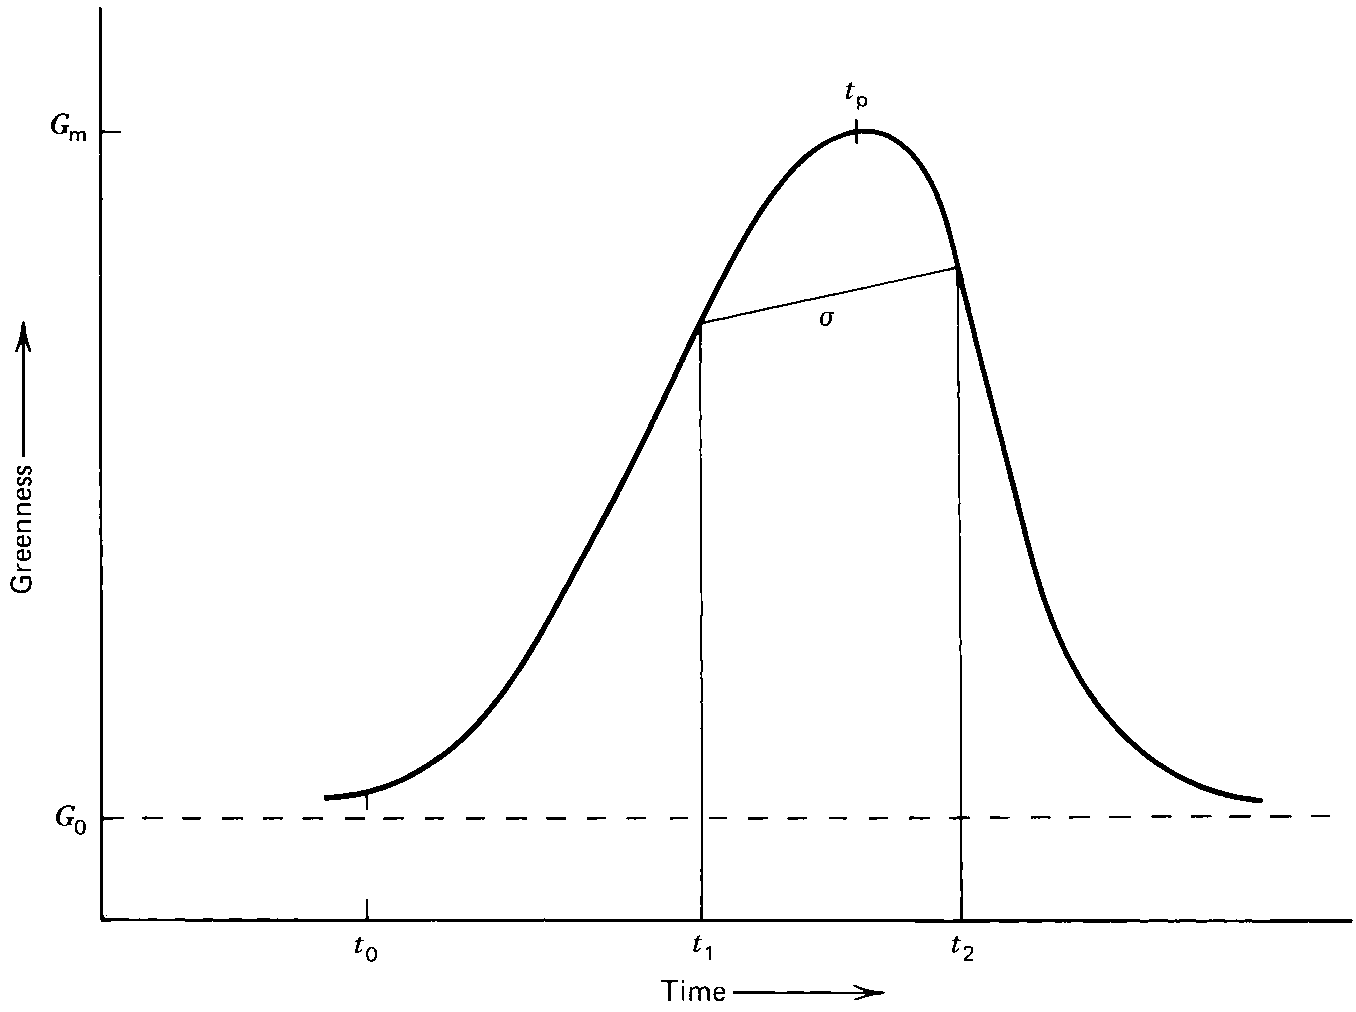
\includegraphics[width=0.7\textwidth]{figures/fig60} \\
    \tiny Key parameters include spectral emergence date ($t_0$), time ($t_p$) of peak greenness ($G_m$), and width of the profile ($\sigma$).
\end{frame}

\subsection{Future Directions}

\begin{frame}{Conclusion: The Data Marathon}
    \begin{itemize}
        \item Time series analysis transforms remote sensing from a ``map-making'' tool into a ``process-monitoring'' tool.
        \item \textbf{Agrophysical Mapping:} Variables like $G_m$ and $t_p$ relate directly to plant health and harvest timing.
        \item \textbf{Scale:} Essential for tracking global change, from desertification to the impact of abnormal flooding.
    \end{itemize}
\end{frame}

\begin{frame}{Homework}
    \begin{itemize}
        \item Pick one of the following papers about the Continuous Change Detection (CCDC) algorithm:
            \begin{enumerate}
                \item Zhu, Z., \& Woodcock, C. E. (2014). Continuous change detection and classification of land cover using all available Landsat data. Remote sensing of Environment, 144, 152-171. \url{https://doi.org/10.1016/j.rse.2014.01.011}

                \item Arévalo, P., Bullock, E.L., Woodcock, C.E., Olofsson, P., (2020). A Suite of Tools for Continuous Land Change Monitoring in Google Earth Engine. Front. Clim. 2. \url{https://doi.org/10.3389/fclim.2020.576740}
            \end{enumerate}
        \item Prepare a reading report following the \LaTeX ~template you will find in the Lab04 folder.
        \item Submit your report (one per student), via Brightspace\texttrademark ~assigment, before class at \textbf{March 19, 2026}.
    \end{itemize}
\end{frame}

\end{document}
